\documentclass{report}
\usepackage{amsfonts}
\usepackage{graphicx}
\graphicspath{./Images/}
\usepackage{amssymb}
\usepackage{physics}
\usepackage{tensor}
\usepackage{hyperref}
\hypersetup{
  colorlinks=true,
  linkcolor=blue,
  filecolor=magenta,      
  urlcolor=cyan,
  pdftitle={Notes},
  pdfpagemode=FullScreen,
}

\author{Jay Rashamiya}
\begin{document}

\begin{titlepage}
  \begin{center}
    \line(1,0){300}\\
    \huge{\bfseries Tricks and Techniques}\\
    \line(1,0){300}\\
    \textsc{\LARGE Jay Rashamiya}\\
    \vspace{5cm}
  \end{center}

  \noindent \textsc{\large I knew a lot of things. Over time, I forgot many things. Now, I only know a few things. Therefore I took the wise decision of noting stuff down. To start, I try to summarize the most elementary things I knew, and the hope is that I'll keep on adding new things that I learn. For now, it's almost all the undergrad stuff which I am trying to summarize as quickly as possible.}
\end{titlepage}

\tableofcontents

\chapter{Magic of Infinitesimals}
\section{Continuity}
\subsection{Any mid value}
\textbf{Statement:} If function $f(x)$ is continuous in the interval $[a,b]$ with $f(a) = A$ and $f(b) = B$, then every value in the interval $[A,B]$ is achieved. Namely, $\forall N \in [A,B], \exists \xi \in [a,b]$ such that $f(\xi) = N$ \\

\noindent\textbf{Proof:} Not required.

\subsection{Max and Min value}
\textbf{Statement:} If the function is continuous in a closed interval than it has a largest and a smallest value for atleast one $x$ in that interval. (Other way of saying that it doesn't become infinite). \\

\noindent\textbf{Use:} In rolle's theorem, for the existence of highest value.

\section{Differentiability}
\subsection{Rolle's Theorem}
\textbf{Statement :} If the function is differentiable in the interval $[a,b]$ and $f(a) = f(b)$, $\exists$ $\xi$ $\in$ $(a,b)$ such that $f'(\xi) = 0$. \\

\noindent\textbf{Proof :} Use sign change/existence argument at maximum.\\

\noindent\textbf{Use :} Finding remainder term in taylor series. Proving L'Hopital rule and various other places where we construct a new function on which we can apply Rolle to prove certain thing about a given function.\\

\subsection{Mean Value theorem}
\textbf{Statemnt :} For a differentiable function in a given interval $[a,b]$, $\exists$ $\xi$ $\in$ $(a,b)$ such that $f'(\xi) = \frac{f(b)-f(a)}{b-a}$ \\

\noindent\textbf{Proof :} Using rolle's theorem.\\

\noindent\textbf{Use :} $f(b) = f(a) + (b-a) f'(a+\theta (b-a))$, $\theta \in [0,1]$.

\subsection{Taylor series}
A function which can be differentiated arbitary number of times can always be expanded as \\\
$$f(b) = f(a) + (b-a)f'(a) + \frac{(b-a)^2}{2!}f''(a) + \dots + \frac{(b-a)^n}{n!}f^{(n)}(a) + R_n$$
The remainder term can be beautifully calculated using rolle's theorem as 

$$R_n = \frac{(b-a)^{n+1}}{(n+1)!} f^{(n+1)}(\xi)$$

\noindent Clearly, this tends to zero as n tends to infinity if the derivative is bounded (which is, because we assumed it exists). A clever trick for finding out taylor series for indefinite integrals is to find the taylor series of integrand and integrate them.

\section{Infinitesimals}
Summing up (infinite times), or dividing is same as summing up (infinite times) or divding only the principal part.\\

\noindent Three properties are important for geometric visualization of calculus:\\

\noindent \textbf{Property 1 :} Any general arc differes from its chord by an infinitestimal of a higher order. Using this, we can imainge arcs as chords (and same extension in higher dimensions, curved surface as planes). We can find the curve length by ignorigng this higher order infinitesimal differnce between arc and chord because infinite sum of infinitesimals is same as infinite sum of their principal parts.\\

\noindent \textbf{Property 2 :} Perpendicular distance from one end of the infintestimal arc to the tangent at the other end  is an infitesimal of higher order than arc, however the length of the tangent from the foot of prependicular to the point of tangency is of the same order. You can prove this by using maclaurine series in transformed coordinates or by simple geometric construction.\\

\noindent \textbf{Property 3 :} Same trigonometric laws are obeyed. This is because the chord becomes tangent to the arc as their length approaches zero. The rules of chord extend to the arcs.

\section{Differentials}

Note that for an independent variable $d^2x = 0$, not otherwise. For independent variable $x$, differential $dx$ is same as infinitesimal increment $\Delta x$ to x. For dependent variable $y$, the differential $dy$ is the principal part of the infinitesimal change $\Delta y$ in $y$. The rules for differentials can easily be derived.

$$\lim_{\Delta x\to 0} \frac{\Delta y}{\Delta x} = f'(x)$$
$$\Delta y = f'(x)\Delta x + \epsilon\Delta x$$
$$dy = f'(x)dx$$

\noindent Knowing usual rules for differnetials, we can use them as algebraic quantities, no need to think of differential operators.\\

\noindent Note the difference between the context of the symbol $\frac{d^2 y}{dx^2}$. Which has context independent meaning only when x is independent variable.\\

\noindent\textbf{Implicit Function Theorem :} If $F(x,y)=0$ and $|F_x| < \infty$ with $F_y\neq 0$, then $y(x)$ exists and is differentiable. Can be easily extended to higher dimensions and/or involving more than one function using jacobians.

\chapter{Sequences}
I list all the theorems which you can prove in order and digest.\\

\noindent\textbf{Defn :} A sequence $(x_n)$ is said to convere to $x$ if $\forall \epsilon > 0$, $\exists N\in \mathbb{N}$ such that $|x_n - x| < \epsilon, \forall n > N.$ \\

\noindent \textbf{Theorem 1 :} If sequence $(x_n)$ converges, it has a unique limit point.\\

\noindent \textbf{Thorem 2 :} If sequence $(x_n)$ converges, it is bounded. (Bounded : $\exists M \in \mathbb{R}$ such that $\forall n,  |x_n| < M$).\\

\noindent \textbf{Theorem 3 :} If a \textbf{monotone} sequence $(x_n)$ is bounded, then it converges. The limit is $sup\{x_n : n \in \mathbb{N}\}$ \\

\noindent \textbf{Theorem 4 :} Every subsequence of a convergent sequence converges to the limit of sequence.\\

\noindent \textbf{Theorem 5 :} Every sequence has a monotone subsequence.\\

\noindent \textbf{Theorem 6 :} (Bolzano) Every bounded sequence has a convergent subsequence. (Just a consequence of prev theorem)\\

\noindent \textbf{Defn :} Limsup/ Liminf of sequence $(a_n)$ are defined by 

$$\limsup_{n\to\infty} a_n = \lim_{n\to\infty}sup(\{a_k : k>=n\})$$ 
$$\liminf_{n\to\infty} a_n = \lim_{n\to\infty}inf(\{a_k : k>=n\})$$ \\

\noindent \textbf{Thoerem 7 :} limsup/liminf of a bounded sequence always exists.\\

\noindent \textbf{Theorem 7 :} Let $(x_n)$ be a bounded sequence. Then $\exists$ subsequences $(x_{n_k})$ and $(x_{m_k})$ s.t.
$$\lim_{n\to\infty}x_{n_k} = \limsup x_n$$
$$\lim_{n\to\infty}x_{n_k} = \liminf x_n$$



\noindent \textbf{Theorem 8 :} If every convergent subsequence of $(x_n)$ has the same limit $x$, then $(x_n)$ converges to $x$.\\

\noindent \textbf{Cauchy Sequence :} A sequence $(x_n)$ is cauchy sequence, if $\forall \epsilon > 0, \exists N \in \mathbb{N}$ such that $|x_n - x_m| < \epsilon , \forall m,n> N$\\

\noindent \textbf{Theorem 9 :} \textbf{A sequence $(x_n)$ converges iff it's a Cauchy sequence.}\\




\chapter{Series}
Same presentation as chapter 2.\\

\noindent \textbf{Defn : }If $(a_n)$ is a a sequence of real numbers then the series $\sum_{n=1}^{\infty}a_n$  converges to $S \in \mathbb{R}$ if the seuqnece $(S_n)$ of partial sum converges to $S$.\\

\noindent \textbf{Trick : } For geometric and telescopic series, you can find explicit formula for $n^{th}$ term of the sequence $(s_n)$.\\

\noindent \textbf{Theorem 1 :} A series $\Sigma a_n$ of positive term converges iff its partial sums are bounded.\\

\noindent \textbf{Theorem 2 :} (Cauchy Condition) The series $\Sigma a_n$ converges iff $\forall \epsilon > 0, \exists N \in \mathbb{N}$ such that $|S_n - S_m| < \epsilon, \forall n > m > N$\\

\noindent \textbf{Defn :} Series $\Sigma a_n$ converges absolutely if $\Sigma |a_n|$ converges. It converges conditionally if $\Sigma a_n$ converges but $\Sigma |a_n|$ diverges.\\

\noindent \textbf{Theorem 4 :} Absolutely convergent series $\Sigma a_n$ converges. Moreover, $\Sigma a_n$ converges absolutely, iff series $\Sigma a_n^{+}$ and $\Sigma a_n^{-}$ converges.\\

Follwoing tests can all be proved simply, using cauchy criterion.\\

\noindent \textbf{Test for divergence :}  If series $\Sigma a_n$ converges, then $\lim_{n\to\infty} a_n = 0$ \\

\noindent \textbf{Comparision test :} If $b_n\ge0, \Sigma b_n$ converges, then $\Sigma a_n$ converges absolutely if $|a_n| \le b_n$\\

\noindent \textbf{Ratio test :} If $(a_n)$ is a sequence of nonzero real numbers, let 
$$ r = \lim_{n\to\infty}\Bigl|\frac{a_{n+1}}{a_n}\Bigr|$$
\noindent Series $\Sigma a_n$ converges absolutely if $0\le r<1$, diverges if $1<r\le \infty$\\

\noindent \textbf{Root test :} For $(a_n)$
$$ r = \lim_{n\to\infty} sup|a_n|^{\frac{1}{n}}$$
\noindent The series converges absolutely if $0\le r<1$ and diverges if $1<r<\infty$.\\

\noindent\textbf{Alternating series test :} If $(a_n)$ is a decreasing sequence of nonnegative real numbers, such that $lim_{n\to\infty}a_n=0$, then the alternating series $\Sigma (-1)^{n+1}a_n$ converges.\\

\noindent\textbf{Limit Comparisiont test :} If $\Sigma a_n$ and $\Sigma b_n$ are two seires and 

$$ r:= \lim_{n\to\infty}\big(a_n/b_n\big) $$

\noindent If $r=0$ : If $\Sigma b_n$ converges, then $\Sigma a_n$ converges.\\
\noindent If $r=\infty$ : If $\Sigma b_n$ diverges, then $\Sigma a_n$ diverges.\\
\noindent IF $r$ is finite, either both converge or both diverge.\\

\noindent\textbf{Theorem 4 :} Every rearrangement of an absolutely convergent series converges to the same sum.\\

\section{Power series :}

There's only one power series for a given funcion (Coefficients are obviously uniquely defined by differentiation).

\begin{itemize}

  \item If a power series converges for some $x=x_1$, it converges absolutely and uniformly for all $|x_2| < |x_1|$. This can be proven using comparision test.\\

    Follwowing are the conseqences of uniform convergence :

    \begin{enumerate}
      \item The function defined by power series is continuous inside the region of convergence. 

      \item The power series can be integrated term by term in the region of convergence.

      \item The power series can be differentiated term by term. This is a more restrictive condition : the continuity of all individual derivatives as well as  the uniform convergence of the series formed by derviative is required.

    \end{enumerate}

  \item On the boundary of region of convergence, there is atleast one singularity.

  \item Laurent Series and Analytic function.

  \item Using residue calculus to sum the series.

\end{itemize}

\chapter{Integration}

\begin{itemize}

  \item Any upper sum will be greater than any lower sum. Infinite integrals (in integrands and in limits) are defined by taking appropriate limits. If function is discontinuous at only finitely many points, both limits approach to the same value, which is defined as the integral

  \item Differentiating under the integral sign. Uniform convergence in $\alpha$ is required for infinite limits.

  \item Integrating under the integral sign is rarely appreciated. Nice trick.

  \item Green's and Stokes theorem (easy proof).

\end{itemize}

\chapter{Complex Variables}

\begin{itemize}

  \item Cauchy reimann conditions for analyticity are sufficient when first order derivatives are also continuous. Analyticity is defined as differentiability in a region. 

  \item As an example $|z|^2$ is differentiable at $z=0$ but not analytic anywhere.

  \item The corresponding real functions of analytic function are harmonic and the conjugate functions form an orthogonal family. Moving along one would give maximum change in the other. The mapping is conformal at point when $f'(z) \neq 0$ or $f'(z) \neq \infty$.

\end{itemize}

\section{Cauchy's Theorem and Integral Formula} If $f(z)$ is analytic in a simply connected region and $C$ is a closed contour in that region then

$$\oint_{C}f(z)dz = 0$$

$$\frac{1}{2\pi i}\oint_{C}\frac{f(z)}{z-z_0}dz = f(z_0)$$

\begin{enumerate}
  \item Taylor and laurent series are simple consequence of this.
  \item Residue is very important for performing various integrals and summing series(as that is the only term that will remain after integration). 
  \item Apart from poles and essential singularity, branch points are also a type of singularity.
  \item for $z^\frac{1}{2}$, the branch point is at $z=0$, order is defined as the number of paths around that point to return to same value. In this case it's $2$.
\end{enumerate}


\section{Analytic Continuation}
In real analysis, a function defined on a given range can be smoothly extended to outer regions in many ways. There's only a unique way to do so for analytic functions. This great property makes complex analysis almost GODLY.\\

\noindent If two analytic functions coincide in any region, or on any finite line segment, they are the same function.


\chapter{Differential Equations}

I won't even mention ODE's with constant coefficients.
\section{First Order ODE}

\begin{itemize}
  \item One can always find integrating factor for first order ODE in principle. In practice, we only know direct formula for \textbf{linear} first order ODE. This also means that every differential constraint (in two dimensions) is holonomic.

  \item List of famous non-linear first order equations that can be solved

    \begin{enumerate}
      \item Bernoulli equation
        $$\frac{dy}{dx} + P(x)y = Q(x)y^n$$
      \item Clairaut's equation
        $$y = x\frac{dy}{dx} + f\left(\frac{dy}{dx}\right)$$
      \item D'Alembert's equation
        $$y = xf\left(\frac{dy}{dx}\right) + g\left(\frac{dy}{dx}\right)$$
    \end{enumerate}

\end{itemize}

\section{Second Order Linear ODE}
Most important differential equations arising in physics are almost always second order and linear (ordinary or partial). Let's consider only the homogenous part right now.
$$y'' + P(x)y' + Q(x) = 0$$

\noindent \textbf{Ordinary Point :} $x_0$ for which $P(x_0)$ and $Q(x_0)$ are finite.\\

\noindent \textbf{Regular Singular Point :} Singular $x_0$ for which $(x-x_0)P(x)$ and $(x-x_0)^2 Q(x)$ remain finite.\\

\noindent \textbf{Irregular Singular Point :} Singular $x_0$ for which one of $(x-x_0)P(x)$ or $(x-x_0)^2 Q(x)$ diverge.\\

\begin{itemize}
  \item The only trick we know is Frobenius! Always check if the final solution converges. You have to expand about a clever point. Expanding about essential singularity won't work.\\

  \item Expressing ODE as $L(x)y(x) = 0$. If $L(x) = L(-x)$, then if $y(x)$ is a solution, so is $y(-x)$. So you can express general solution as a linear combination of odd and even.
\end{itemize}

\noindent \textbf{Wronskian :} To test for linear independence of functions, we obtain $n$ equations by differentiating the relation 

$$\sum_{i=0}^{n}a_i \phi_i (x) = 0$$

\noindent This is the origin of Wronskian! Also used in some ninja-technical way to find particular solution for inhomogenous linear equation.

\subsection{Sturm-Liouville Theory}

In physics, we don't really require general solutions. We require solutions with specific boundary conditions. Specific boundary conditions impose conditions on the parameters of the equation. For instance, for a string clamped at $x=0$ and $x=l$, in the differential equation $\frac{d^2\psi}{dx^2} + k^2\psi(x) = 0$ , $k$ will have certain restrictions as you know. Here, $k^2$ is the eigenvalue.\\

\noindent Charecterization of general features of eigenproblems arising \textbf{from linear second-order differential equations} is known as Strum-Liouville theory.\\

\noindent Consider $\mathcal{L}\psi(x) = \lambda\psi(x)$, where

$$\mathcal{L}(x) = p_0(x)\frac{d^2 \psi}{dx^2} + p_1(x)\frac{d\psi}{dx} + p_2(x)$$

\noindent Now $\mathcal{L}$ is known as self adjoint if $p_0'(x) = p_1(x)$, which enables us to write 

$$\mathcal{L}(x) = \frac{d}{dx}\left[p_0(x)\frac{d}{dx}\right]+p_2(x)$$

\noindent We can show that

$$\int_{a}^{b}v^*(x)\mathcal{L}u(x)dx = \left[v^* p_0 u' - (v^*)'p_0 u\right]_{a}^{b} + \int_{a}^{b}(\mathcal{L}v)^* u dx$$

\begin{itemize}
  \item Dirichlet Boundary : $u$ and $v$ both vanish at endpoints.
  \item Neumann Boundary : $u'$ and $v'$ both vanish at endpoints.
  \item Any second order linear operator can be turned into Sturm-Liouville form by changing the scalar product to include weight factor.
\end{itemize}

\noindent If $u$ and $v$ are eigenfunctions of $\mathcal{L}$ with respective eigenvalues $\lambda_u$ and $\lambda_v$, then we can see that they are orthogonal. \textbf{This is great beacause we have just proven orthogonality of Trigonometric, Bessel, Legendre, Hermite, Laguerre, Chebyshev. Further, completeness of eigenfunctions is the origin of fourier series!}\\

\noindent Namely, if $f(x)$ satisfy boundary conditions of Sturm-Liouville and is continous and piecewise differentiable on $[a,b]$ then eignefunction expansion of $f$ converges uniformly to $f$ on $[a,b]$. If it's piecewise differentiable, then it converges to $[f(x_+) + f(x_-)]/2$ on $[a,b]$.

\noindent To solve, inhomogenous strum lioville equation, we solve the eigenequation of the given operator with given boundary condition, which allows us to find the eigenfunction expansion of the inhomogenous equation.

\subsection{Special Functions and Polynomials}

A summary of results about special functions can be found \href{https://webspace.science.uu.nl/~hooft101/lectures/specialfct.pdf}{Here}

\subsection{Variational Method}
Suppose that the spectrum of the hamiltonian $H$ has a finite greatest lower bound. In such cases, we have a simple yet very powerful method to guess the ground state energy and wavefunction.


$$\expval{H}{\Psi} \ge E_0$$

\noindent This allows us to guess a paramaterized wavefunction and choose the parameter which minimizes the expectation value. The result can only get better because the ground state has lowest energy among all such $\psi$


\section{Partial Differential Equations}
Second order (mostly linear, but even non-linear) partial differential equations are everywhere. It's all of physics. 

\subsection{Charecteristic}
Understanding boundary conditions is important. Consider for example a simple first order PDE

$$\mathcal{L}\phi = a\frac{\partial\phi}{\partial x} + b\frac{\partial\phi}{\partial y} = 0$$

\noindent We generally try to change variables in such a manner that the equation reduces to something which only contains derivative w.r.t one term. Here $s = ax+br, t= bx-ay$ does the job. Reducing it to 

$$\frac{\partial\phi}{\partial s} = 0 \quad\implies \phi(x,y) = f(bx-ay)$$

\noindent Observe that the solution is constant along constant $t$. It is known as the charecterisic curve. It's not necessary that solution remains constant on charecteristic cuve, but it can be solved using ODE methods on the charecteristic curve. If $\phi(x,y)$ is specified on a curve segment, one can deduce its value on all the charecteristics that intersects it.

$$\phi(x,y) = \phi(x_0,y_0) + \frac{\partial \phi(x_0,y_0)}{\partial x}(x-x_0) + \frac{\partial\phi(x_0,y_0)}{\partial y}(y-y_0) + ...$$

\noindent We can obtain the values of partial derivatives using the equations determining the curve and the given partial differential equation (Arfken p.405).\\

\noindent If the boundary curve is along a charecteristic, then there may be inconsistencies. IF the boundary intersects same charecteristic on more than one point, then it may lead to inconsistencies as well.\\

\noindent Exact general analysis of boundary conditions is complicated. Look up when you need it. For reference of three simple yet important PDE's\\

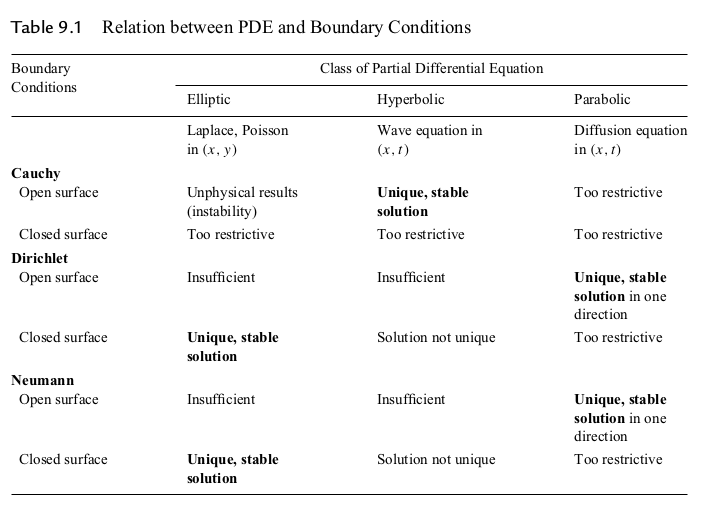
\includegraphics[width=10cm, height=7cm]{./Images/boundary.png}

\section{Integral Transforms}
Due to integration by parts, we can change derivatives to algebraic equations by integral transforms. Additionally, we have shifting property to receive answers modulo exponential.

\subsection{Fourier Transform}

\subsection{Laplace Transform}

\subsection{Legendre Transformation}
A function $f(x,y)$ can be seen as a function $g$ of $u$ and $y$ by certain transformation. (Note : $u=\frac{\partial f}{\partial x}$)

$$g = f - ux$$

\noindent This is key to going from lagrangian formalism to hamiltonian.

\section{Dirac Delta}
Any sequence of function, whose integral over all space is unity and it vanishes for all points except at zero as $n$ goes to $\infty$ will converge to dirac delta function. Extremely useful in quantum field theory.

\begin{enumerate}
  \item $\delta(x) = \frac{1}{2\pi}\int_{-\infty}^{\infty} e^{ikx} dk $
\end{enumerate}

\chapter{Asymptotics and Perturbation Methods}

$\lim_{x\to x_0} \frac{f(x)}{g(x)} = 1 := f(x) \sim g(x) \quad\mathrm{as}\quad  x\to x_0$\\

\noindent$\lim_{x\to x_0} \frac{f(x)}{g(x)} = 0 := f(x) << g(x)\quad\mathrm{as}\quad  x\to x_0$\\


\noindent Given an asymptotic sequence(each successive term having lower order) $\{\phi_i\}$ The coefficients of the assymptotic expansion 

$$ f(x) \sim a_1\phi_1(x) + a_2\phi_2(x) + ... $$

\noindent are uniquely determined.\\

\noindent If the remainder term is of lower order than the last term of the expansion for all $n$, the exapnsion is called asymptotic.\\

\noindent $\bold{Caution 1:}$ Two given functions differing by transcendentally small terms (exponentials as compared to powers) can have same asymptotic expansions. Hence, these terms are ignored in asymptotic expnsions (in powers of $x$). TST are related to essential singularities.\\

\noindent $\bold {Caution 2:}$ Need to keep higher order terms in exponentials (including sin,cos,sinh,cosh etc). Not doing so, can give wrong prefactor.\\

\noindent $\bold{Caution 3:}$ Differentiating can cause trouble too. Look at ``Tauberian Theorems" (BO - p.127)

\section{For Integrals}

\subsection{Integration by Parts}

\noindent In general, if we have

$$I(x) = \int_{a}^{b} f(t) e^{x\phi(t)} dt \quad\mathrm{as}\quad x\to\infty$$ 

$$I(x) = \int_{a}^{b} \frac{f(t)}{x\phi'(t)} d(e^{x\phi(t)})$$

$$I(x) = \frac{1}{x} \left[\frac{f(t)}{\phi(t)} e^{x\phi'(t)}\right]_{t=a}^{t=b} - \frac{1}{x}\int_{a}^{b}\frac {d}{dt}\left[\frac{f}{\phi'}\right]e^{x\phi(t)}dt $$

We hope that the second integral has lower order than the first term and that $\phi'(t)$ is not zero anywhere in the interval. This will fail when asymptotic expansion involves $log$ or fractional powers of $x$.

\subsection{Laplace's Method}

For ``sharply-peaked" integrands, where the dominant contribution comes from the nbd of a single point, we can expand the function involved in exponent around that point.\\

\noindent $\bold{Example 1 :}$

$$ I(x) = \int_{-10}^{10}e^{-xt^2}dt \quad\mathrm{as}\quad x\to\infty$$

\noindent Integration by parts won't work because $\phi'(0) = 0$. Dominant contribution comes for $t=0$. 

$$I(x) = \int_{-\infty}^{\infty}e^{-xt^2}dt - 2\int_{10}^{\infty}e^{-xt^2}dt$$

\noindent First part is simple gaussian integral, we can estimate the second integral by replacing $t^2$ bt $10t$. Which will show that the second term is transcendentally smaller than the first term.

$$I(x) \sim \sqrt{\frac{\pi}{x}}$$

\noindent $\bold{Stirling's Approximation :}$

$$\Gamma(x+1) = \int_{0}^{\infty}t^x e^{-t}dt$$

\noindent Where's the peak of this integrand ? 

$$ \Gamma(x+1) = \int_{0}^{\infty}e^{x\log(t)-t}dt$$

\noindent Maximum occurs when the exponent is maximized, which gives $x = t$. Maximum moves with $x$. We change coordinates where it doesn't change. Define $ s = \frac{t}{x}$

$$\Gamma(x+1) = x^{x+1}\int_{0}^{\infty}e^{x\log(s) - s}ds$$

\noindent Expanding $\log$ about $s=1$.

$$\Gamma(x+1) \sim x^{x+1}\int_{0}^{\infty}e^{-x\left(1+\frac{(1-s)^2}{2}\right)}ds$$

$$\Gamma(x+1) \sim x^{x+1}e^{-x}\int_{0}^{\infty}e^{-x\frac{(1-s)^2}{2}}ds$$

\noindent We can't do this integral. But if we add TST, we have usual gaussian integral!

$$\Gamma(x+1) \sim x^{x+1}e^{-x} \sqrt{\frac{2\pi}{x}}$$

\subsection{Stationary Phase}

For an integral of the function $f(t)$ multiplied with an oscillating function, we get cancellations. If the frequency of oscillation is sufficiently big, we expect the integral to vanish. Rigorously speaking :

$$I(x) = \int_{a}^{b}f(t)e^{ix\psi(t)}dt$$

\noindent As $x\to\infty$, we try integration by parts to get


$$I(x) = \left[\frac{f(t)e^{ix\psi(t)}}{ix\psi'(t)}\right]_{t=a}^{t=b} - \frac{1}{ix}\int_{a}^{b}\frac{d}{dt}\left[\frac{f}{\psi'}\right]e^{ix\psi(t)}$$

\noindent Again, just hoping for usual conditions on $\psi'(t)$ and the second integral being of lower order, we see that 

$$I(x) \sim O\left(\frac{1}{x}\right)$$

\noindent At points when $\psi'(t) = 0$, the first order oscillation of $\psi$ vanishes, meaning it oscillates much more slowely (in second order of $t$) near this point. It gives a contribution of higher order than $O(\frac{1}{x})$. Therefore, we only integrate near neighbourhood of that point of stationary phase. After expanding around that point, a standard trick would be then to extend this region to infinity, if corresponding integral is easy to do. Since this extension would contribute to higher order terms only.

\noindent Expanding around the stationary phase ($\psi'(c) =0 $), and using Fresnel's integral(really just use Gamma function formula), we can show that if 

$$\mathrm{if}\quad f^{(i)}(c) = 0 \quad\forall i<n \quad \mathrm{then} \quad  I(x) \sim O\left(\frac{1}{x^{\frac{1}{n}}}\right)$$

\noindent A useful way to think about both the laplace and stationary phase method in a coherent manner is to see that the function multiplying $f(t)$ has an exponential order. Meaning they change much faster than $f(t)$ as long as $f(t)$ doesn't have exponential order. Note that complex representation of sin and cosine make this evident for this oscillatory functions as well. In some sense then, the integral is wholly dominated by this exponential ordered terms (including sine,cosine). Therefore we only care about the regions where this exponential ordered terms are slowly varying (given that they decay eventually in case of laplace method). In laplace method, it was the peak. In stationary phase method, it is the stationary phase.\\

\noindent \textbf{Bessel function}\\

$$J_0(x) = \frac{1}{\pi}\int_{0}^{\infty}\cos(x\sin(t)) dt$$

\noindent $\psi'(t) = 0$ at $t=\frac{\pi}{2}$. Expanding $\sin(t)$ about $t=\frac{pi}{2}$

$$\sin\left(t\right) = \sin\left(\frac{\pi}{2}\right) + \cos\left(\frac{\pi}{2}\right)\left(t-\frac{\pi}{2}\right) -\frac{1}{2}\sin\left(\frac{\pi}{2}\right)\left(t-\frac{\pi}{2}\right)^2 + ...$$

$$\mathrm{As}\quad x\to\infty$$ 
$$\frac{1}{\pi}\int_{0}^{\pi}e^{ix\sin(t)}dt\sim \frac{1}{\pi}\int_{\frac{\pi}{2}-\epsilon}^{\frac{\pi}{2}+\epsilon}e^{ix\left[1-\frac{1}{2}\left(t-\frac{\pi}{2}\right)^2 +...\right]}dt$$

\noindent As done again and again, expanding the limits of integration because it only affects higher order terms, we get 

$$J_0\left(x\right) \sim \sqrt{\frac{2}{\pi x}} \cos\left(x-\frac{\pi}{4}\right) \quad\mathrm{as}\quad x\to\infty$$

\subsection{Steepest Descent}
This method makes previous two methods a consequence. Consider the integral 

$$I(x) = \int_{C}h(t)\, e^{x\phi(t)}\, e^{ix\psi(t)}$$

\noindent If we choose a contour such that the $\psi(t)$ is constant on this contour, we can bring it out of the integral and use laplace's method. This will enable us to find higher order terms that we missed in stationary phase method. Please check the video by Professor Strogatz for example.\\

\chapter{Groups}

\section{Finite Groups}

\noindent\textbf{Once and Only Once Rule:} In the multiplication table, each row or each column contains each element of the group exactly once. Try constructing all posible finite groups of order n.\\

\noindent\textbf{Lagrange's Theorem:} Order of every subgroup divides the order of original group. (Using disjointness of cosets)\\

\noindent\textbf{Centre:} The set defined by elements $z_i$ such that $z_i$ commutes with all elements of the group is an abelian subgroup of $G$.\\

\noindent\textbf{Permutations:} A permutation can be decomposed into product of two cycles. It's even or odd depending on number of two cycles present. (Imagine the ball hiding guy arranging the glasses. He achieves all sort of permutation by doing exchanges again and again). Odd and even because matrix representation corresponds to elementary operations which have determinants $1$ or $-1$.\\

\noindent\textbf{Cayley's Theorem:} Any finite group $G$ with $n$ elements is isomorphic to a subgroup of $S_n$ (Permutation Group). (Associate each $g_i$ with corresponding permutation by checking the permutation offered by observing the multiplication table.)\\

\noindent\textbf{Conjugation:} Two elements $g$ and $g'$ are similar if there exists an element $f$ such that $f^{-1}gf = g'$. Conjugation is an equivalence relation, therefore we can form equivalence classes. (Doing something, doing main thing, undoing something leads to a similar element in some sense. Which is what defines this relation). Equivalence classes provide disjoint partitions of the set (Simple proof). Equivalence relations provide a zoom out lens of a given set.\\

\noindent\textbf{Invariant Subgroup:} Say $H$ is a group. Conjugate $H$ with some $g$ not in $H$. It will give another group. Conjugation will lend to similar elements but not same. If the conjugated group is same as the original group \textbf{for all g}. Then that group is special, and rightly deserves the name Invariant subgroup. All elements equivalent to elements in the subgroup $H$ are also in $H$.\\

\noindent\textbf{Quotient Group:} If $G$ has an invariant subgroup $H$, we can form another group consisting of left cosets $g_aH$ as elements called the Quotient group $G/H$. We can zoom out sets using equivalence relation, in the same way we need invariant subgroups to zoom out of the group if we want to preserve the group strucutre. It's a somewhat stronger condition than just using equivalence class to zoom out in order to keep group structure. \\

\section{Rotations and Lie Algebra}

Calculus is mankind's greatest invention. We analyze behaviours of functions in infinitesimal neighbourhood and then form differential equations to find the right relationship (from infinitesimals to reals). Taylor series is, in a sense $f(x+\Delta x) = exp(\Delta x\frac{d}{dx})f(x)$. For groups, the higher derivatives $\frac{d^n}{dx^n}$ are simple matrix multiplication of the generator $\frac{d}{dx}$. Rotation is defined by

$$R^{T}R = I \quad det(R) = 1$$

\noindent Check that generators are antisymmetric matrices. We stick in $-i$ to make the generators hermitian.

\subsection{Lie Algebra}

Instead of looking at the actual elements of the group, we are now concerned with generators only. We can go back to the actual group using exponention. For instance, $SO(n)$ generators are antisymmetric matrices. A general antisymmetric matrix can be seen as linear combination of $\frac{n(n-1)}{2}$ antisymmetric matrices. \\

\noindent The commutativeness of the original group elements is related to the commutation relation of the generator. Commutation relation of the generators form an algebra which is called lie algebra of the cooresponding lie group.

$$[J_i, J_j] = i\epsilon\indices{_i_j_k}J_k$$

\noindent We can do something like this for all sorts of lie groups. Where $\epsilon$ are repaced by some other constants known as the structure cosntatnts.

\section{Representation Theory}

It's useful to represent the group elements $g$ as matrices which preserve the multiplication structure of the group. Namely,

$$D(g_1 g_2) = D(g_1)D(g_2)$$

\noindent Obviously, $D(g) = 1$ (one dimensional identity matrix) is a perfectly good representation. There's a loss of information in some sense. $D$ is homomorphism as is written, but if it is an isomorphism, we say that the representation is faithful (useful). Since every finite group is a subgroup of $S_n$, and $S_n$ has obvious representation of dimension $n$, we have faithful representations of every finite group. (A bit complicated for continuous groups, but we're physicists)

\subsection{Character is a function of class}

$$\chi^{(r)}(g) = Tr(D^{(r)}(g))$$

\noindent There may be many representations of the same group. We denote a particular representation $r$ by $D^{(r)}$. Character of a particular element under a given representation is the trace of $D^{(r)}(g)$ , and is denoted by $\chi^{(r)}(g)$. It's easy to prove that \textbf{character of an entire equivalence class is same.} (Using cyclic property of trace).

\subsection{Equivalent represntation} 

There may be more than one representation of a given group. Clearly, We are only concerned with reducible representations. Even among the reducible representations, given a representation $D(g)$, we can construct another representation $D'(g) = S^{-1} D(g) S$ (check that $D'$ is really a presentation). These representations are esentially the same connected by similarity transformation. If we are given two represenations, are they same? One thing you can check is that the character is invariant under the representations connected by similarity transformation. Therefore, if each matrix was conjugated (similarly transformed) and we were to be presented with weird looking set of matrices as representation, they may just be realted to some simple looking set of matrices via similarity transformation.

\chapter{Theory of Lie}

All functions considered are smooth etc. $x$ without subscript inside the function is to be seen as something which involves all $x_i$. Imagine a flat space and cartesian coordinates of dimension $n$. Now consider, a set of transformations (Called point transformation)

$$x'_i = f_i(x_1, x_2, x_3, ...) \quad \forall i \in {1,2,..n}$$

\noindent We can imagine $x$ moving to $x'$ in the same system or a region in the domain of $x$ system being mapped to a correesponding region of $x'$ system.\\

\noindent We wish to see this transformation as a continous group. What do we need? We want it to be invertible. Which demands usual condition of Jacobian being non-zero under the region of consideration. Further, if we were to transform twice using different parameters, we should end up in the same family. Let's introduce a notation for finite parameter continuous group to make this more clear. \\

\noindent A continuous transformation involving finite parameters will be represented as $x' = f(x;a)$. For this family to form a group, we demand that $x'' = f(x'; b) = f(x;c)$. Now if we have a $r$ parameter transformation 

$$x'_i = f_i(x_1,x_2,...; a_1,a_2,...,a_r)$$

\noindent We can eliminate the constants to form a set of differential equations for $x'_i$. This differential equations will have an amazing property. Namely, if we find two different set of families of solution $x'_i = g_i(x;b_1,b_2,...,b_r)$ and $x'_i = h_i(x;a)$. Then the composition $y'_i = g_i(h_1(x,a), h_2(x,a),...;b_1,b_2,...,b_r)$ is also a solution by definition of the group property of initial equation.\\

\noindent A function $f$ in $x$ system may look very different in $x'$ system. If it looks the same, we say that the trasformation which takes $x$ to $x'$ is a symmetry of $f$. The magic in theory of continuous groups is that we can always analyze upto the first order near identity, namely, we are dealing with generators only. An explicit example is considered below (Section of Killing Vectors).\\

\noindent More generally, let $x$ be transformed to $y$ and $u_i(x)$ be transformed to different functions under the group action, which in $y$ coordinates, have the form $v(y)$, then the function $P(x,\frac{\partial u}{\partial x}, \frac{\partial ^2 u}{\partial x^2},...)$ is an invariant of the group if 

$$ P\left(x,\frac{\partial u}{\partial x}, \frac{\partial ^2 u}{\partial x^2},...\right) = P\left(y,\frac{\partial v}{\partial y}, \frac{\partial ^2 v}{\partial y^2},...\right)$$


\section{Killing vectors}

Consider finding out symmetries of the metric in relativity. We consider an infinitesimal transformation at all coordinates

$${x'}\indices{^\mu} = x\indices{^\mu} + \epsilon \, \eta\indices{^\mu}(x)$$

\noindent Here, $\eta\indices{^\mu}(x)$ is like $dx\indices{^\mu}$, hence it can be treated as vector. Namely, its indices can be lowered and uppered. Note also, that the inverse transformation can be given by (since first order change inside the function $\eta$ will give second order overall change)


$$x\indices{^\mu} = {x'}\indices{^\mu} - \epsilon \, \eta\indices{^\mu}(x')$$

\noindent The metric transforms under general coordinate transformation as 

$${g'}\indices{_\alpha_ \beta}(x') = g\indices{_\mu _\nu}(x)\frac{\partial x\indices{^\mu}}{\partial {x'}\indices{^\alpha}} \frac{\partial x\indices{^\nu}}{\partial {x'}\indices{^\beta}}$$

\noindent We want the metric to keep the same form under such coordinate transformation, meaning that we want ${g'}\indices{_\alpha_ \beta}(x') = g\indices{_\alpha_ \beta}(x')$. This connects the $x$ system and $x'$ system in a sense. Equation says that the point $x$(system 1) in the manifold which is also the point $x'$(system 2) in different system is related to the point $x'$(system 1) of the original system in this fashion. 

$$g\indices{_\alpha_ \beta}(x) + \epsilon \, \partial_\sigma g\indices{_\alpha_ \beta} \, \eta\indices{^\sigma}(x)= g\indices{_\mu_ \nu}(x) \left[\delta\indices{^\mu_\alpha} -\epsilon \, \partial_\alpha\eta\indices{^\mu}\right] \left[\delta\indices{^\nu_ \beta} -\epsilon \, \partial_ \beta\eta\indices{^\nu}\right]  $$

\noindent Here, we have ignored $\epsilon^2$ terms arising from partial derivatives of $\eta$ evaluated at infinitesimally different point. Which will give us a coordinate independent equation for vector $\eta\indices{^\mu}$

$$\nabla\indices{_\mu}\eta\indices{_\nu} + \nabla\indices{_\nu}\eta\indices{_\mu} = 0 $$

\noindent The vector field $\eta$ is then the generator of the continuous symmetry of the metric.

\subsection{A brief note on invariance}

There's a deep but trivial connection between the coordinate transformation that preserve the form of the function and the symmetry of the function. This very connection is the reason for noether's theorem. As stressed many times, Transformation we will consider are infinitesimal (Finite can be generated easily from them).\\

\noindent Say we have a new coordinate system $x' = x + \epsilon \, \eta(x)$. Any function $f(x)$ will have a totally different form $f'(x')$. Here, $x$ and $x'$ refer to the same point on the manifold, but in different coordinate systems. Hence, the numerical value of two expression is same $f'(x') = f(x)$. However, if we want the form of the function itself to be the same in new coordinate system, we need $f'(x') = f(x')$. But if the transformation $x'=x'(x)$ is such that $f(x') = f(x)$ then we clearly have $f'(x') = f(x')$. Such transformation for which $f(x') = f(x)$ correspond to the infinitesimal symmetry of the function. Therefore, transformation which are the symmetry of the function are also the same transformation which preserve the form of the function under coordinate transformation. It's trivial, but took me long to realise.

\chapter{Quantum Mechanics}

\begin{itemize}

  \item A state of quantum system is defined by a ket $\ket{\psi}$ or the corresponding bra $\bra{\psi}$ (For every vector space, we can construct a dual space (of linear functionals)). There is a one-one correspondence between this space.

  \noindent \textbf {Pedantry} : If $V$ is a finite dimensional vector space, its dual $V^*$ has the same dimension. Therefore, they're isomorphic. (Note that finite dimensional vector spaces with same dimensions are obviously isomorphic.) By establishing the dual basis, we establish this isomorphism between $V$ and $V^*$. But this isomorphism is not natural. However, if we have an inner product space, we can have almost natural isomorphism between a vector $\ket{\alpha}$ and its dual, $\bra{\alpha}$ is naturally defined by fixing the first element of inner product as $\ket{\alpha}$.

  \item Inner product is positive definite and has conjugate symmetry by defintion. Important for probabilistic interpreation :
    $$\bra{\alpha}\ket{\beta} = \bra{\beta}\ket{\alpha}^* \quad \textrm{and} \quad \bra{\alpha}\ket{\alpha} \ge 0$$ 

  \item The eigenvalues of a Hermitian operator ar ereal and Eigenkets corresponding to different eigenvalues are orthogonal. Every observable corresponds to a Hermitian operator. Converse, I am not aware of yet. \\

  \textbf{Postulate:} The eigenkets of an observable are complete. This is a physical requirement, not a mathematical truth. As a consequence, we start by identifying the observables, and since they're hermitian, we choose an orthonormal basis consisting of eigenkets of this observable, which will span the entire hilbert space.

\item If $[A,B] = 0$, we they've same, every eigenvector of $A$ is an eigenvector of $B$.

\item Given two sets of base kets ${\ket{a^{(i)}}}$ and ${\ket{b^{(i)}}}$, there is a unitary operator

  $$U = \sum_{k} \ket{b^{(k)}}\bra{a^{(k)}}$$

  such that $\ket{b^{(i)}} = U\ket{a^{(i)}}$

  Check $U^\dag U = I$

\item Matrix representation of the operator $X$ changes in different bases by a similarity transformation $X' = U^\dag XU$, where $X, U, X'$ are now seen as matrices, not operators. 


\end{itemize}


\chapter{General Relativity}
No better summary than Dirac's 60 page book. Roughly speaking, $\partial_\mu$ can be treated as a vector direction if one imagines $y^n$ to be accompanied with it. Also explains how it changes if surface is not flat or the coordinates are curved.

\begin{itemize}
  \item An observer is a worldine where the basis vector he chooses at each point of the worldline reduces the metric to $\eta\indices{_a_b}$. In effect, he's someone who uses flat metric at all points of the worldline. (Schuller Lect 13. 41:26)

  \item All momentum components $p\indices{^\mu}$ are not independent due to reparameterization invariance of the lagrangian. In classical mechanics, time was a thing which was used to define action. (David Tong p.22 GR).


  \item In 2 dimesnions, gaussian curvature is sufficient to describe inner properties of the space. In higher dimensions, we need more.


    \begin{enumerate}
      \item Metric can be chosen at a point such that $g\indices{_\mu_\nu}(P) = \eta\indices{_\mu_\nu}$ and $\Gamma\indices{^\alpha_\beta_\gamma}(P) = 0$ (Poisson p.27)

      \item Suppose $P\indices{_\mu_\nu_\lambda}$ is such that $A\indices{^\mu}P\indices{_\mu_\nu_\lambda}$ is a tensor for any vector $A\indices{^\mu}$. Then $P\indices{_\mu_\nu_\lambda}$ is a tensor. Useful for quickly proving something is a tensor.
      
      \item $\Gamma\indices{^\alpha_ \beta_ \gamma} = \frac{1}{2}g\indices{^\alpha^\lambda}\left[\partial_ \gamma g\indices{_ \lambda_ \beta} + \partial_ \beta g\indices{_\lambda_ \gamma}-\partial_\lambda g\indices{_ \beta_ \gamma}\right]$
      \item
        $\nabla\indices{_\mu}A\indices{^\nu} = \partial_{\mu}A\indices{^\nu} + \Gamma\indices{^\nu_\lambda_\mu}A\indices{^\lambda}$
      \item
        $\nabla\indices{_\mu}A\indices{_\nu} = \partial_{\mu}A\indices{_\nu} - \Gamma\indices{^\lambda_\nu_\mu}A\indices{_\lambda}$ \\
        For general tensors, use leibniz rule. $g\indices{_\mu_\nu}$ can be treated as a constant under covariant derivative.

      \item $\nabla\indices{_ \rho}\nabla\indices{_\sigma}A\indices{_\nu} - \nabla\indices{_\sigma}\nabla\indices{_ \rho}A\indices{_ \nu} = A\indices{_ \lambda}R\indices{^\lambda_\nu_ \rho_\sigma}$

      \item $R\indices{^\beta_\nu_ \rho_\sigma} = \partial_ {\rho}\Gamma\indices{^\beta_\nu_\sigma}-\partial_ {\sigma}\Gamma\indices{^\beta_\nu_\rho} + \Gamma\indices{^\alpha_\nu_\sigma} \Gamma\indices{^\beta_ \alpha_ \rho} - \Gamma\indices{^\alpha_\nu_ \rho} \Gamma\indices{^\beta_ \alpha_ \sigma}$

    \end{enumerate}
\end{itemize}


\end{document}
